\documentclass[svgnnames,dvipsnames]{standalone}

\usepackage[dvipsnames=xcolor]{xcolor}

\usepackage{tikz}
\usetikzlibrary{positioning,shadows.blur}
\usepackage{pifont} %?

\renewcommand{\labelitemi}{\ding{112}} %?

\begin{document}

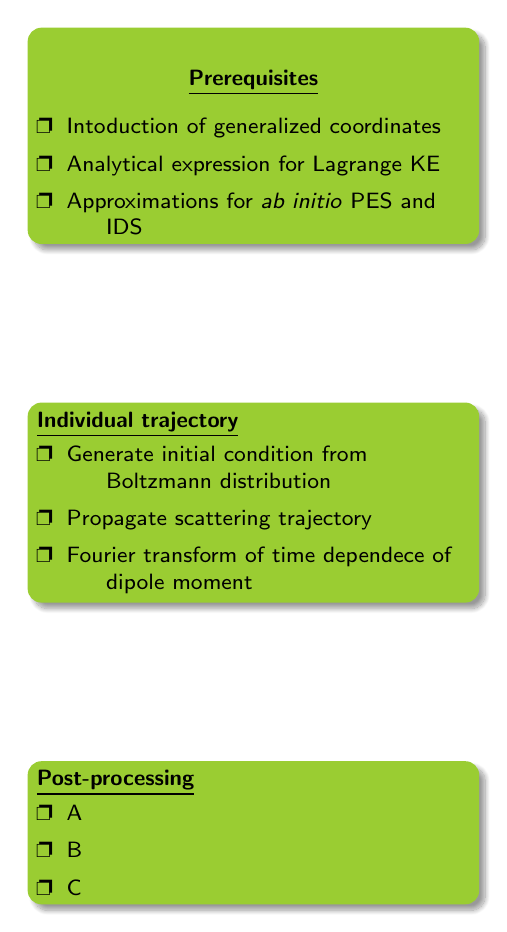
\begin{tikzpicture}
   \tikzset{
     box/.style    = { rounded corners = 5pt,
                       align           = left,
                       font            = \sffamily\footnotesize,
                       text width      = 5.5cm, 
                       blur shadow     = {shadow blur steps = 15} },    
     legend/.style = { font       = \sffamily\bfseries, 
                       align      = right,
                       text width = 3.4cm},
  }

  \iffalse
  \node [shade,
    blur shadow  = {shadow blur steps = 15},
    text width   = 1.01\textwidth,
    top color    = black, 
    bottom color = Maroon,
    text         = white, 
    font         = \sffamily\bfseries\large] (A)
    {Aggregates, global feedback dynamics, ...  \\ \vspace{.6\textwidth} 
    Individual objects, exact sizes, distances, velocities, timings, ...};
  
  \node [box, below left  = -4.5cm and -3.85cm of A, fill = YellowGreen]
    (DE)
    {\underline{\bfseries Discrete Event (DE)}
      \begin{itemize} 
        \setlength{\itemindent} {-.5cm}
        \item entities (passive objects)
        \item flowcharts 
        \item network ressources
      \end{itemize}
    };
  \fi
  
    \node [box, fill = YellowGreen ] (Initial)
        {
            \begin{center} \underline{\bfseries Prerequisites} \end{center}
            \begin{itemize}
                \setlength{\itemindent} {-.5cm}
                \item Intoduction of generalized coordinates
                \item Analytical expression for Lagrange KE 
                \item Approximations for \textit{ab initio} PES and IDS 
            \end{itemize}
        };

    \node [box, fill = YellowGreen, below = 2cm of Initial] (Cycle)
        {   
            \underline{\bfseries Individual trajectory}
            \begin{itemize}
                \setlength{\itemindent} {-.5cm}
                \item Generate initial condition from Boltzmann distribution
                \item Propagate scattering trajectory
                \item Fourier transform of time dependece of dipole moment
            \end{itemize}
        };

    \node [box, fill = YellowGreen, below = 2cm of Cycle] (Cycle)
        {   
            \underline{\bfseries Post-processing}
            \begin{itemize}
                \setlength{\itemindent} {-.5cm}
                \item A
                \item B
                \item C
            \end{itemize}

        };


\end{tikzpicture}
\end{document} 
